\documentclass{standalone}
\usepackage{tikz}
\usetikzlibrary{patterns, positioning}
\usepackage[sfdefault]{ClearSans} %% option 'sfdefault' activates Clear Sans as the default text font
\usepackage[T1]{fontenc}

\begin{document}
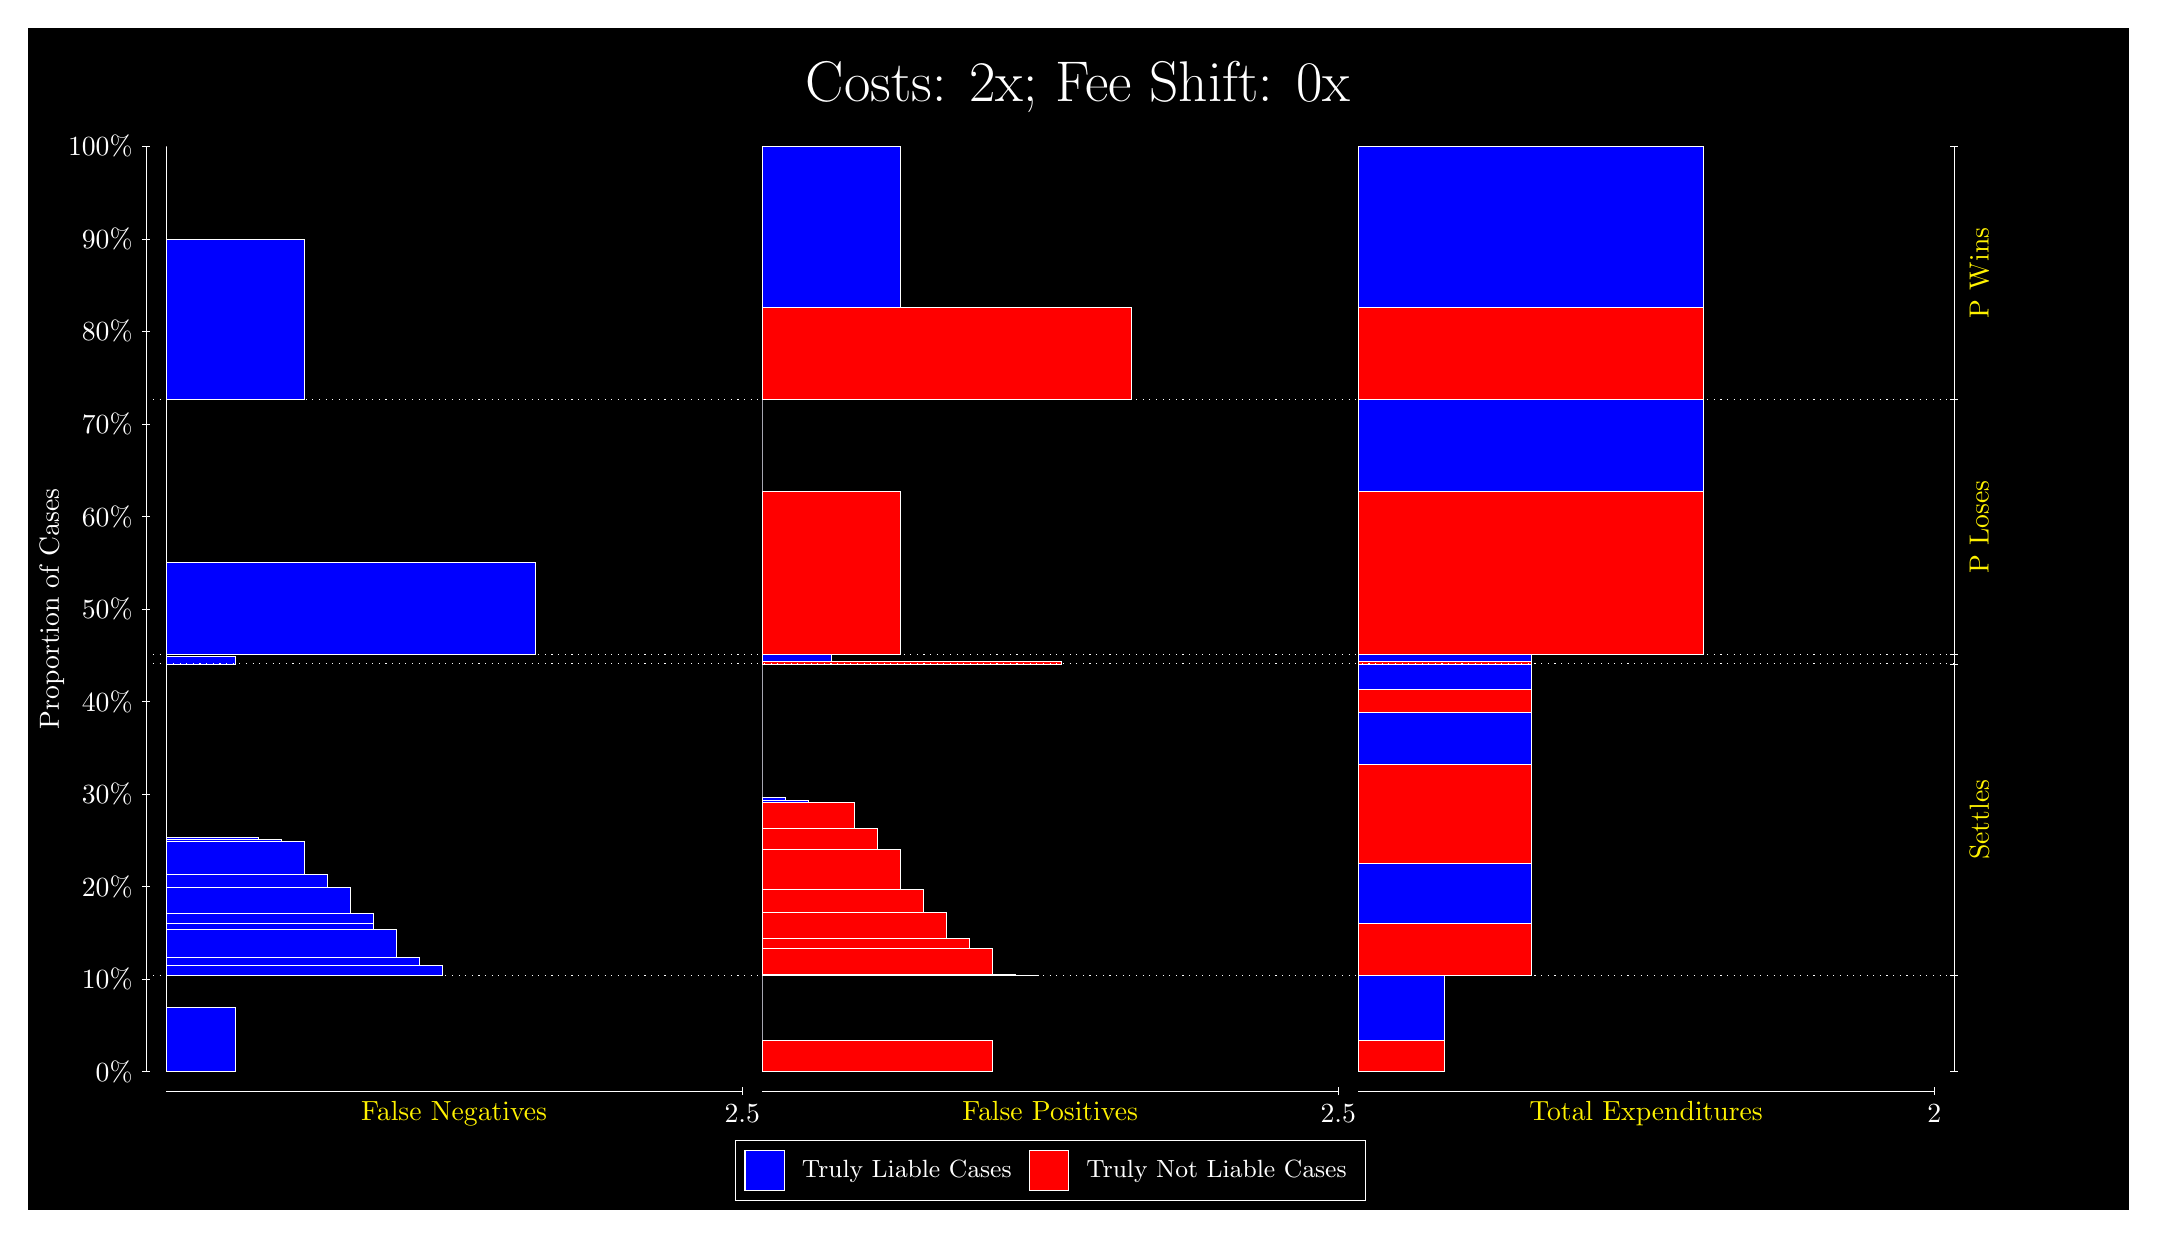
\begin{tikzpicture}
\draw[fill=black] (0,0) rectangle (26.667,15);
\draw[text=white] (0,13.5) rectangle (26.667,15) node[midway] {\huge Costs: 2x; Fee Shift: 0x};
\draw[white, very thin] (1.5,1.75) -- (1.5,13.5);
\node[rotate=90, text=white, anchor=center] at (0.3, 7.625) {Proportion of Cases};
\draw[white, very thin] (1.45,1.75) -- (1.55,1.75);
\node[text=white, anchor=east] at (1.45, 1.75) {0\%};
\draw[white, very thin] (1.45,2.925) -- (1.55,2.925);
\node[text=white, anchor=east] at (1.45, 2.925) {10\%};
\draw[white, very thin] (1.45,4.1) -- (1.55,4.1);
\node[text=white, anchor=east] at (1.45, 4.1) {20\%};
\draw[white, very thin] (1.45,5.275) -- (1.55,5.275);
\node[text=white, anchor=east] at (1.45, 5.275) {30\%};
\draw[white, very thin] (1.45,6.45) -- (1.55,6.45);
\node[text=white, anchor=east] at (1.45, 6.45) {40\%};
\draw[white, very thin] (1.45,7.625) -- (1.55,7.625);
\node[text=white, anchor=east] at (1.45, 7.625) {50\%};
\draw[white, very thin] (1.45,8.8) -- (1.55,8.8);
\node[text=white, anchor=east] at (1.45, 8.8) {60\%};
\draw[white, very thin] (1.45,9.975) -- (1.55,9.975);
\node[text=white, anchor=east] at (1.45, 9.975) {70\%};
\draw[white, very thin] (1.45,11.15) -- (1.55,11.15);
\node[text=white, anchor=east] at (1.45, 11.15) {80\%};
\draw[white, very thin] (1.45,12.325) -- (1.55,12.325);
\node[text=white, anchor=east] at (1.45, 12.325) {90\%};
\draw[white, very thin] (1.45,13.5) -- (1.55,13.5);
\node[text=white, anchor=east] at (1.45, 13.5) {100\%};

\draw[white, very thin] (24.457,1.75) -- (24.457,13.5);
\draw[white, very thin] (24.407,1.75) -- (24.507,1.75);
\node[anchor=west] at (24.407, 1.75) {};
\draw[white, very thin] (24.407,2.9694) -- (24.507,2.9694);
\node[anchor=west] at (24.407, 2.9694) {};
\draw[white, very thin] (24.407,6.9274) -- (24.507,6.9274);
\node[anchor=west] at (24.407, 6.9274) {};
\draw[white, very thin] (24.407,7.0497) -- (24.507,7.0497);
\node[anchor=west] at (24.407, 7.0497) {};
\draw[white, very thin] (24.407,10.286) -- (24.507,10.286);
\node[anchor=west] at (24.407, 10.286) {};
\draw[white, very thin] (24.407,13.5) -- (24.507,13.5);
\node[anchor=west] at (24.407, 13.5) {};

\draw[white, very thin, fill=blue] (1.75,1.75) rectangle (2.6283,2.5703);
\draw[white, very thin, fill=red] (1.75,2.5703) rectangle (1.75,2.9694);
\draw[white, very thin, fill=blue] (1.75,2.9694) rectangle (5.2631,3.0958);
\draw[white, very thin, fill=blue] (1.75,3.0958) rectangle (4.9703,3.2032);
\draw[white, very thin, fill=blue] (1.75,3.2032) rectangle (4.6775,3.5542);
\draw[white, very thin, fill=blue] (1.75,3.5542) rectangle (4.3848,3.6345);
\draw[white, very thin, fill=blue] (1.75,3.6345) rectangle (4.3848,3.7631);
\draw[white, very thin, fill=blue] (1.75,3.7631) rectangle (4.092,4.0896);
\draw[white, very thin, fill=blue] (1.75,4.0896) rectangle (3.7993,4.2605);
\draw[white, very thin, fill=blue] (1.75,4.2605) rectangle (3.5065,4.6689);
\draw[white, very thin, fill=blue] (1.75,4.6689) rectangle (3.2138,4.7018);
\draw[white, very thin, fill=blue] (1.75,4.7018) rectangle (2.921,4.728);
\draw[white, very thin, fill=red] (1.75,4.728) rectangle (1.75,6.9274);
\draw[white, very thin, fill=blue] (1.75,6.9274) rectangle (2.6283,7.0196);
\draw[white, very thin, fill=red] (1.75,7.0196) rectangle (1.75,7.0497);
\draw[white, very thin, fill=blue] (1.75,7.0497) rectangle (6.4341,8.2161);
\draw[white, very thin, fill=red] (1.75,8.2161) rectangle (1.75,10.286);
\draw[white, very thin, fill=blue] (1.75,10.286) rectangle (3.5065,12.323);
\draw[white, very thin, fill=red] (1.75,12.323) rectangle (1.75,13.5);
\draw[white, very thin, fill=red] (9.3189,1.75) rectangle (12.246,2.1491);
\draw[white, very thin, fill=blue] (9.3189,2.1491) rectangle (9.3189,2.9694);
\draw[white, very thin, fill=red] (9.3189,2.9694) rectangle (12.832,2.9763);
\draw[white, very thin, fill=red] (9.3189,2.9763) rectangle (12.539,2.9883);
\draw[white, very thin, fill=red] (9.3189,2.9883) rectangle (12.246,3.3167);
\draw[white, very thin, fill=red] (9.3189,3.3167) rectangle (11.954,3.4467);
\draw[white, very thin, fill=red] (9.3189,3.4467) rectangle (11.661,3.7698);
\draw[white, very thin, fill=red] (9.3189,3.7698) rectangle (11.368,4.0668);
\draw[white, very thin, fill=red] (9.3189,4.0668) rectangle (11.075,4.5736);
\draw[white, very thin, fill=red] (9.3189,4.5736) rectangle (10.783,4.8334);
\draw[white, very thin, fill=red] (9.3189,4.8334) rectangle (10.49,5.1688);
\draw[white, very thin, fill=blue] (9.3189,5.1688) rectangle (9.9044,5.195);
\draw[white, very thin, fill=blue] (9.3189,5.195) rectangle (9.6116,5.2279);
\draw[white, very thin, fill=blue] (9.3189,5.2279) rectangle (9.3189,6.9274);
\draw[white, very thin, fill=red] (9.3189,6.9274) rectangle (13.125,6.9575);
\draw[white, very thin, fill=blue] (9.3189,6.9575) rectangle (10.197,7.0497);
\draw[white, very thin, fill=red] (9.3189,7.0497) rectangle (11.075,9.1192);
\draw[white, very thin, fill=blue] (9.3189,9.1192) rectangle (9.3189,10.286);
\draw[white, very thin, fill=red] (9.3189,10.286) rectangle (14.003,11.462);
\draw[white, very thin, fill=blue] (9.3189,11.462) rectangle (11.075,13.5);
\draw[white, very thin, fill=red] (16.888,1.75) rectangle (17.986,2.1491);
\draw[white, very thin, fill=blue] (16.888,2.1491) rectangle (17.986,2.9694);
\draw[white, very thin, fill=red] (16.888,2.9694) rectangle (19.083,3.6329);
\draw[white, very thin, fill=blue] (16.888,3.6329) rectangle (19.083,4.4008);
\draw[white, very thin, fill=red] (16.888,4.4008) rectangle (19.083,5.6516);
\draw[white, very thin, fill=blue] (16.888,5.6516) rectangle (19.083,6.3167);
\draw[white, very thin, fill=red] (16.888,6.3167) rectangle (19.083,6.6019);
\draw[white, very thin, fill=blue] (16.888,6.6019) rectangle (19.083,6.9274);
\draw[white, very thin, fill=red] (16.888,6.9274) rectangle (19.083,6.9575);
\draw[white, very thin, fill=blue] (16.888,6.9575) rectangle (19.083,7.0497);
\draw[white, very thin, fill=red] (16.888,7.0497) rectangle (21.279,9.1192);
\draw[white, very thin, fill=blue] (16.888,9.1192) rectangle (21.279,10.286);
\draw[white, very thin, fill=red] (16.888,10.286) rectangle (21.279,11.462);
\draw[white, very thin, fill=blue] (16.888,11.462) rectangle (21.279,13.5);
\draw[white, dotted] (1.5,2.9694) -- (24.457,2.9694);
\draw[white, dotted] (1.5,6.9274) -- (24.457,6.9274);
\draw[white, dotted] (1.5,7.0497) -- (24.457,7.0497);
\draw[white, dotted] (1.5,10.286) -- (24.457,10.286);
\draw[white, very thin] (1.75,1.5) -- (9.0689,1.5);
\node[text=yellow, anchor=north] at (5.4094, 1.5) {False Negatives};
\draw[white, very thin] (9.0689,1.45) -- (9.0689,1.55);
\node[text=white, anchor=north] at (9.0689, 1.45) {2.5};

\draw[white, very thin] (9.3189,1.5) -- (16.638,1.5);
\node[text=yellow, anchor=north] at (12.978, 1.5) {False Positives};
\draw[white, very thin] (16.638,1.45) -- (16.638,1.55);
\node[text=white, anchor=north] at (16.638, 1.45) {2.5};

\draw[white, very thin] (16.888,1.5) -- (24.207,1.5);
\node[text=yellow, anchor=north] at (20.547, 1.5) {Total Expenditures};
\draw[white, very thin] (24.207,1.45) -- (24.207,1.55);
\node[text=white, anchor=north] at (24.207, 1.45) {2};


\node[text=yellow, centered, rotate=90] at (24.777, 4.9484) {Settles};

\node[text=yellow, centered, rotate=90] at (24.777, 8.6677) {P Loses};
\node[text=yellow, centered, rotate=90] at (24.777, 11.893) {P Wins};

\draw (12.978300999999998,1.5) node[draw=none] (baseCoordinate) {};
\begin{scope}[align=center]
        \matrix[scale=0.5, draw=white, below=0.5cm of baseCoordinate, nodes={draw}, column sep=0.1cm]{
            \node[rectangle, draw, minimum width=0.5cm, minimum height=0.5cm, fill=blue] {}; &
            \node[draw=none, font=\small, text=white] (B) {Truly Liable Cases}; &
            \node[rectangle, draw, minimum width=0.5cm, minimum height=0.5cm, fill=red] {}; &
            \node[draw=none, font=\small, text=white] (B) {Truly Not Liable Cases}; \\
            };
\end{scope}

\end{tikzpicture}
\end{document}